\documentclass[11pt]{article}
\usepackage{graphicx,epstopdf}
\usepackage{mathpazo}
\usepackage{amsmath,amssymb,fancyvrb,tikz,epstopdf,subfigure}
\usetikzlibrary{positioning}
\usepackage[margin=1in]{geometry}
\newcommand{\ansbox}[1]{%
	\begin{center}
		\tikz{\node[draw,rectangle]{%
			$\displaystyle#1$};}
	\end{center}
}

\newcommand{\p}[2]{\frac{\partial#1}{\partial#2}}

\begin{document}

\begin{flushright}
Cameron Bracken\\
CVEN 5343\\
PS \#3
\end{flushright}

\begin{enumerate}

%%%%%%%%%%%%%%%%%%%%%%%%%%%%%%%%%%%%%
%%%%%%%%%%%%%%%%%%%%%%%%%%%%%%%%%%%%%
\item[1. a)] 

The solution will be the same as the shifted point source, integrated from $-L$ to $L$

$$C(x,t) = \int_{-L}^L\frac{2LC_0}{\sqrt{4\pi Dt}}\exp\left[{\frac{-(x-\xi)^2}{4Dt}}\right]d\xi.$$

Let $$u=\frac{x-\xi}{\sqrt{4Dt}}$$ 
and $$du=\frac{-1}{\sqrt{4Dt}}d\xi$$
so when
$$\xi=L,\,\,\,\,\,u=\frac{x-L}{\sqrt{4Dt}}$$
and when
$$\xi=-L,\,\,\,\,\,u=\frac{x+L}{\sqrt{4Dt}}.$$

The solution then becomes

\begin{align}
C(x,t)&=\frac{-2LC_0}{\sqrt{\pi}}\int_{(x+L)/\sqrt{4Dt}}^{(x-L)/\sqrt{4Dt}}e^{-u^2}du\nonumber\\
&=\frac{-2LC_0}{\sqrt{\pi}}\left[\int_0^{(x-L)/\sqrt{4Dt}}e^{-u^2}du-\int_0^{(x+L)/\sqrt{4Dt}}e^{-u^2}du\right]\nonumber
\end{align}

\ansbox{C(x,t)=-C_0\left[\mbox{erf}\left(\frac{x-L}{\sqrt{4Dt}}\right)-\mbox{erf}\left(\frac{x+L}{\sqrt{4Dt}}\right)\right]}

%%%%%%%%%%%%%%%%%%%%%%%%%%%%%%%%%%%%%
%%%%%%%%%%%%%%%%%%%%%%%%%%%%%%%%%%%%%
\item[1. b)] 

After the peak concentration of the point source has dropped to the initial concentration of the slug then the solutions should look similar. 

$$C(0,t)=C_0=\frac{M}{\sqrt{4\pi Dt}}$$
$$t=\frac{M^2}{4\pi DC_0^2}$$

and since $C_0=M/L$

\ansbox{t=\frac{L^2}{\pi D}}

The solutions indeed look similar at this time:

\begin{figure}[!htbp]
   \centering
   \includegraphics[width=\textwidth]{profs.eps} 
   \caption{Profiles at $t=L^2/(\pi D)$, the shape of the two profiles is indeed similar and the value at $x=0$ is similar.}
\end{figure}

%%%%%%%%%%%%%%%%%%%%%%%%%%%%%%%%%%%%%
%%%%%%%%%%%%%%%%%%%%%%%%%%%%%%%%%%%%%
\item[1. c)] 

Add an image source to the soulution of 1 a) which has an initial profile from $-5L$ to $-3L$.

\ansbox{C(x,t)=-C_0\left[\mbox{erf}\left(\frac{x-L}{\sqrt{4Dt}}\right)-\mbox{erf}\left(\frac{x+L}{\sqrt{4Dt}}\right)\right]-C_0\left[\mbox{erf}\left(\frac{x+3L}{\sqrt{4Dt}}\right)-\mbox{erf}\left(\frac{x+5L}{\sqrt{4Dt}}\right)\right]}

\begin{figure}[!htbp]
   \centering
   \includegraphics[width=\textwidth]{wall1.eps} 
   \caption{Profiles when a wall is placed at $x=-2L$.}
\end{figure}

%%%%%%%%%%%%%%%%%%%%%%%%%%%%%%%%%%%%%
%%%%%%%%%%%%%%%%%%%%%%%%%%%%%%%%%%%%%
\item[1. d)]

The solution when there is a wall at $x=0$ is identical to the solution from part a, except that there will be two of them (one for each side).  The added image source for either side, is the same term as when there is no wall and one continuous profile. 

%%%%%%%%%%%%%%%%%%%%%%%%%%%%%%%%%%%%%
%%%%%%%%%%%%%%%%%%%%%%%%%%%%%%%%%%%%%
\clearpage
\item[2. a)]  

Start with the solution for the 1-D case in the $y$ direction (along $x=x_0$)

$$C(y,t) = \frac{M}{\sqrt{4\pi Dt}}\exp\left[{\frac{-y^2}{4Dt}}\right]$$

and let $M=\dot{M}dx/t$ and $t=x/u$,  then divide by $dx$ to get the 2-D concentration

$$C(x,y) = \frac{\dot{M}}{\sqrt{4\pi Dxu}}\exp\left[{\frac{-y^2u}{4Dx}}\right].$$

Unit check:

$$\frac{M/T}{\sqrt{(L^/T)(L)(L/T)}}=\frac{M/T}{\sqrt{L^4/T^2}}=\frac{M}{L^2}$$

%%%%%%%%%%%%%%%%%%%%%%%%%%%%%%%%%%%%%
%%%%%%%%%%%%%%%%%%%%%%%%%%%%%%%%%%%%%
\item[2 b)]~

\begin{figure}[!htbp]
   \centering
   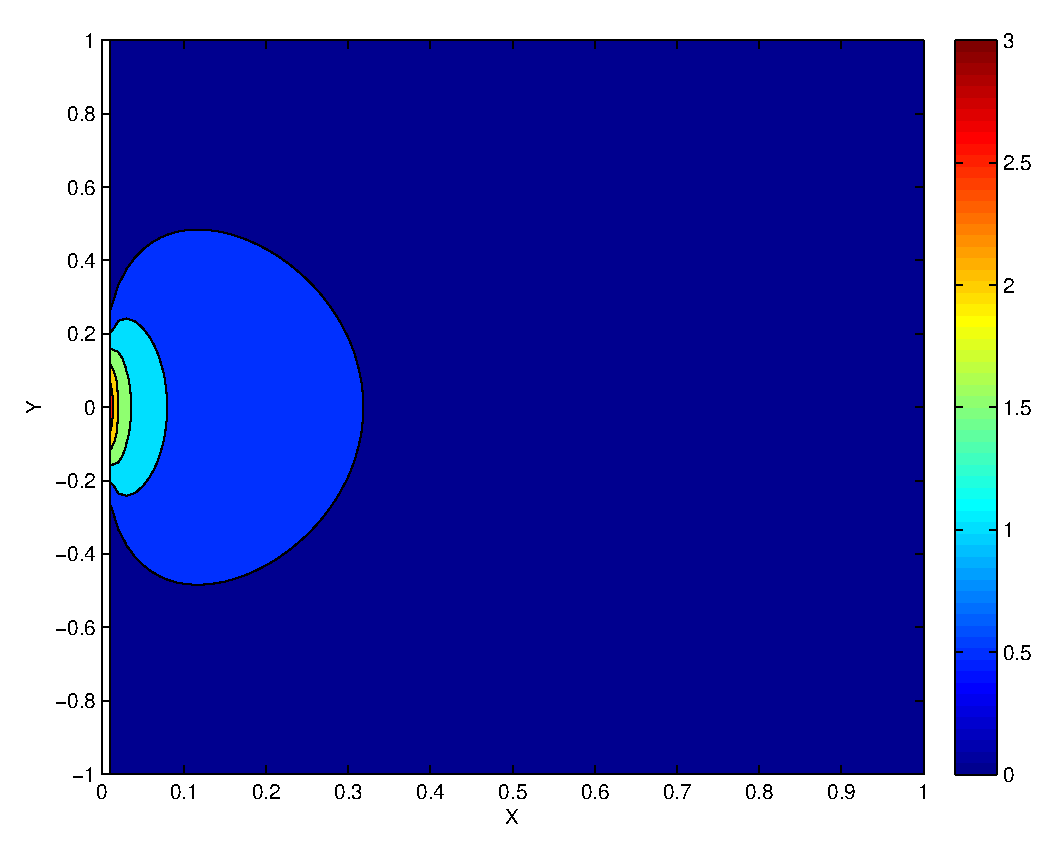
\includegraphics[width=.75\textwidth]{plume2d-contour.eps}
\end{figure}
\begin{figure}[!htbp]
	\centering
	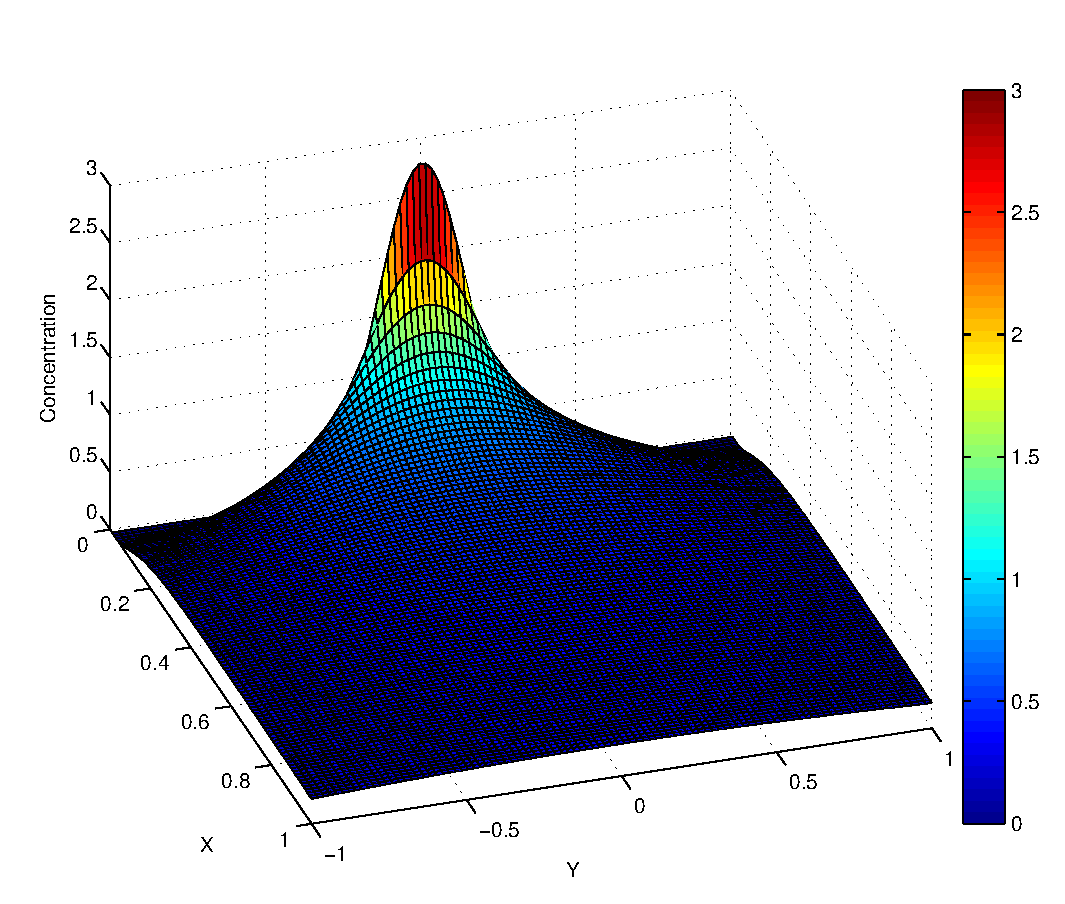
\includegraphics[width=.75\textwidth]{plume2d-surf.eps}
	\caption{Two views of a steady state 2-D plume.}
\end{figure}

\clearpage
%%%%%%%%%%%%%%%%%%%%%%%%%%%%%%%%%%%%%
%%%%%%%%%%%%%%%%%%%%%%%%%%%%%%%%%%%%%
\item[2 c)]

We need to integrate over $y$ to get the total concentration. Let 
$$\theta=\frac{y\sqrt{u}}{\sqrt{4Dx}}$$ 
and $$du=\sqrt{\frac{u}{4Dx}}dy$$

so that

\begin{align}
C_{total}=\int^\infty_{-\infty}C(x,y)dy &= \frac{\sqrt{4Dx}}{\sqrt{4\pi Dxu}\sqrt{u}}\int_{-\infty}^\infty e^{-\theta^2}d\theta\nonumber\\
&=\dot{M}/u
\end{align}

The total advective flux in the x-direction is 

$$q_{adv}=C_{total}u$$ 

so

\ansbox{q_{adv}=\dot{M}}

%%%%%%%%%%%%%%%%%%%%%%%%%%%%%%%%%%%%%
%%%%%%%%%%%%%%%%%%%%%%%%%%%%%%%%%%%%%
\item[2 d)]

Start with the full conservative 2-D A-D equation, 

$$\p{c}{t}+\p{}{x}(uC)+\p{}{y}(uC)+\p{}{x}\left(-D\p{C}{x}\right)+\p{}{y}\left(-D\p{C}{y}\right)=0$$

\begin{itemize}
\item Assume steady state so $\p{C}{t}=0$.
\item Assume no lateral velocity so $\p{}{y}(uC)=0$.
\item Neglect diffusion in the direction of the bulk flow. That is, assume $\p{}{x}(uC) \gg \p{}{x}\left(-D\p{C}{x}\right)$.
\end{itemize}

Then we have 

$$\p{}{x}(uC)+\p{}{y}\left(-D\p{C}{y}\right)=0$$

\clearpage
%%%%%%%%%%%%%%%%%%%%%%%%%%%%%%%%%%%%%
%%%%%%%%%%%%%%%%%%%%%%%%%%%%%%%%%%%%%
\item[2 e)]
~
\begin{figure}[!h]
\centering
	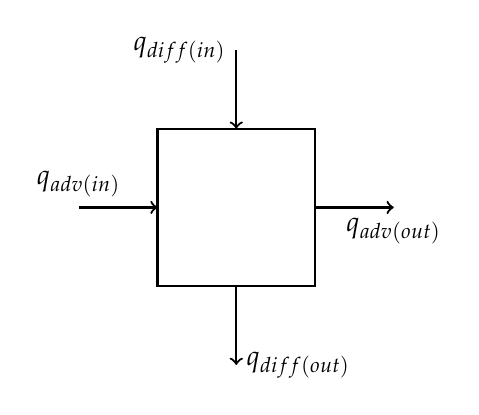
\begin{tikzpicture}
		\draw[thick] (-1,-1) rectangle (1,1);
		\draw[thick,->] (1,0) -- (2,0)  node[anchor=north] {$q_{adv(out)}$};
		\draw[thick,<-] (0,1) -- (0,2) node[anchor=east] {$q_{diff(in)}$};
		\draw[thick,<-] (-1,0) -- (-2,0) node[anchor=south] {$q_{adv(in)}$};
		\draw[thick,->] (0,-1) -- (0,-2) node[anchor=west] {$q_{diff(out)}$};
	\end{tikzpicture}
\caption{2-D Element}
\end{figure}

Streamwise advective flux coming in is balanced by diffusive flux leaving perpendicular to the flow and advective flux leaving. A mass balance gives

$$q_{adv(in)} + q_{diff(in)} = q_{adv(out)} + q_{diff(out)}$$
$$q_{adv(out)} - q_{adv(in)} = q_{diff(out)} - q_{diff(in)}$$

%%%%%%%%%%%%%%%%%%%%%%%%%%%%%%%%%%%%%
%%%%%%%%%%%%%%%%%%%%%%%%%%%%%%%%%%%%%
\item[2 f)]~

\begin{figure}[!h]
\centering
	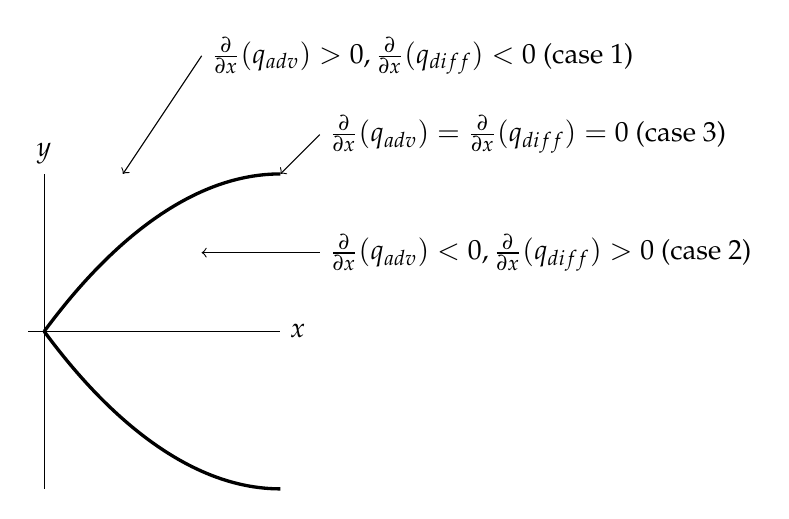
\begin{tikzpicture}
		%\filldraw[color=blue,fill opacity=.5] (0,0) rectangle (3,2);
		%\filldraw[color=orange,fill opacity=.5] (0,0) rectangle (3,-2);
		\draw (0,-2) -- (0,2)node[anchor=south] {$y$};
		\draw (-.2,0) -- (3,0) node[anchor=west] {$x$};
		\draw[very thick] (0,0) parabola[bend at end] (3,2);
		\draw[very thick] (0,0) parabola[bend at end] (3,-2);
		\draw[<-] (3,2) -- (3.5,2.5) node[anchor=west] {$\p{}{x}(q_{adv})=\p{}{x}(q_{diff})=0$ (case 3)};
		\draw[<-] (2,1) -- (3.5,1) node[anchor=west] {$\p{}{x}(q_{adv})<0,\p{}{x}(q_{diff})>0$ (case 2)};
		\draw[<-] (1,2) -- (2,3.5) node[anchor=west] {$\p{}{x}(q_{adv})>0,\p{}{x}(q_{diff})<0$ (case 1)};
	\end{tikzpicture}
\end{figure}

Inside the plume (depends on our tolerance), case (2) holds. The change in the diffusive flux is positive and the change in the advective flux is negative.  Outside of the plume, case (1) holds, the change in the advective flux is positive and the change in the diffusive flux is negative. Along the plume dividing line, fluxes in and out from both diffusion and advection are balanced so case (3) holds. 

%%%%%%%%%%%%%%%%%%%%%%%%%%%%%%%%%%%%%
%%%%%%%%%%%%%%%%%%%%%%%%%%%%%%%%%%%%%
\item[2 g)]

\begin{align}
\mbox{2-D:}\,\,\,\,\,\, C&(x,0) = \frac{\dot{M}}{\sqrt{4\pi Dxu}}\nonumber\\
\mbox{3-D:}\,\,\,\,\,\, C&(x,0,0) = \frac{\dot{M}}{4\pi Dx}\nonumber
\end{align}

The 2-D case diffuses faster near $x=0$ because the gradient in only the two dimensions is larger, not distributed among three dimensions.  The 3-D case diffuses more farthur away from $x=0$ as the mass spreads out ans has more surface area over which to diffuse.


\end{enumerate}

\end{document}  



